\documentclass[runningheads]{llncs}
\usepackage[T1]{fontenc}
\usepackage{pgfplots}
\pgfplotsset{width=10cm,compat=1.9}
\usepackage{tikz}
\usetikzlibrary{matrix,shapes,arrows,positioning}

\begin{document}

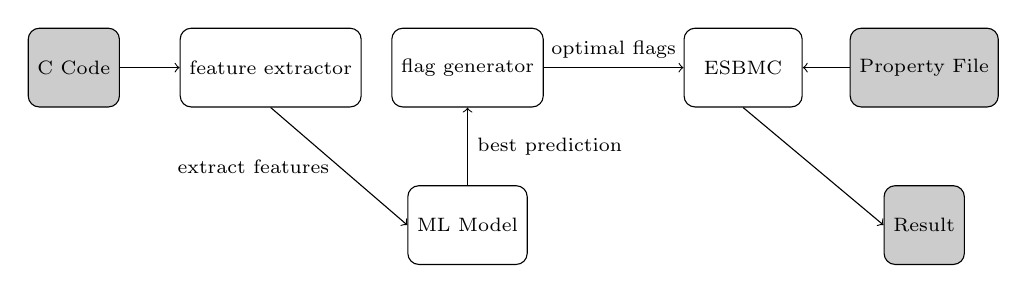
\begin{tikzpicture}[node distance=2cm]
\tikzstyle{io} = [rectangle, rounded corners, minimum width=1cm, minimum height=1cm, text centered, draw=black, fill=black!20]
\tikzstyle{obj} = [rectangle, rounded corners, minimum width=1.5cm, minimum height=1cm, text centered, draw=black]
\tikzstyle{arrow} = [thick,->,>=stealth]
\node (ccode) [io]{\scriptsize C Code};
\node (frontend) [obj, right of = ccode, xshift=0.5cm] {\scriptsize feature extractor}; 
\node (flaggenerator) [obj, right of =frontend,  xshift=0.5cm]{\scriptsize flag generator};
\node (model) [obj, below of= flaggenerator]{\scriptsize ML Model}; 
\node (esbmc) [obj, right of= flaggenerator, xshift = 1.5cm]{\scriptsize ESBMC}; 
\node (property) [io, right of=esbmc, xshift=0.3cm]{\scriptsize Property File};
\node (out) [io, below of=property]{\scriptsize Result};
\draw[->] (ccode.east) -- (frontend.west);
\draw[->] (frontend.south) -- node[anchor=east]{\scriptsize extract features}(model.west);
\draw[->] (model.north) -- node[anchor=west]{\scriptsize best prediction} (flaggenerator.south);
\draw[->] (flaggenerator.east) -- node[anchor=south]{\scriptsize optimal flags} (esbmc.west);
\draw[->] (property.west) -- (esbmc.east);
\draw[->] (esbmc.south) -- (out.west);
\end{tikzpicture}

\end{document}